\section{Improvements ideas}
\label{sec:discussion}
ADOP\cite{ruckert2022adop} is overall an excellent paper. It does not bring so much novel ideas but makes a considerable engineering effort to apply the core idea of NPBG \cite{Aliev2020} to large real scenes.

\noindent \textbf{Focusing only on real scenes.}
Suprisingly, the authors do not mention any attempts to apply their method to synthetic scenes, like the NERF paper initially did and they mention that training a new scene requires a large amount of compute. This could mean they developped their method progressively on a few toy examples and didn't bother releasing results of these tiny examples. Or their method may simply not perform too well on synthetic scenes... which may include a lot of specular materials. Classical NERF test samples scenes usually contain a lot of specular materials where the rendering would most probably fail. I still think it would be beneficial to have a few synthetic scenes to test on including to make quick tests without the need of A100 40Gb trained for several hours.
On the other hand, since the main method's contribution are refining pose estimation (requiring the approximate differentiable aspect of the renderer) and the camera photo simulator, it's not surprising that they'd work on natural photos rather than simulation. 

\noindent \textbf{Camera pipeline module.} 
Their analyzis on this part does not look complete in my humble opinion and looks more like a workaround on having scenes shot with auto-exposure. They picked the low hanging fruits: take care of most exposure changes to end up improving the metrics on the available benchmark (Table 4. from their paper shows that ADOP is better by a large margin than all other algorithms except the M60 tanks scene which has been shot in manual frozen exposure). Their claim to handle the camera imaging pipeline properly and adapt to it is fully justified in the paper but it has a major caveat: results may crumble in case of a more complex camera ISP \footnote{Image Signal Processor}.

Simulating a realistic camera pipeline (like mimicking the ISP which goes from 12bit linear RAW bayer data to a 8 bit jpg) is probably as difficult as correcting first order errors introduced by the camera's ISP as part of the optimization process...Despite the effort on the ablation study (table 3 and figure 6 of \cite{ruckert2022adop}), problem is that we don't really know the exact impact of compensating the camera photo pipeline on the final reconstruction result, at least compared to a scene imaged with perfect ideal linear HDR camera. For instance, they're able to get a sky with cyan shift which looks like the camera picture (they fit the tone mapper correctly).

If we carefully look at the Tanks and Temples dataset \cite{Knapitsch2017TanksAndTemples}, pictures are frames extracted from a mp4 video from 2 different high end cameras, sometimes using auto-exposure. Although it's a good initiative for researchers to keep on using fixed established benchmarks, Tanks and Temples was initially designed for 3D reconstructions (e.g. evaluate performances of Structure from motion like COLMAP estimation compared to a groundtruth lidar captured point cloud) rather than novel view synthesis. The idea is interesting but it will most probably fail with a modern smartphone camera which use local tone mappers and sometimes adapt colors locally.

\label{sec:remplementation}
\begin{figure}[H]
    \centering
    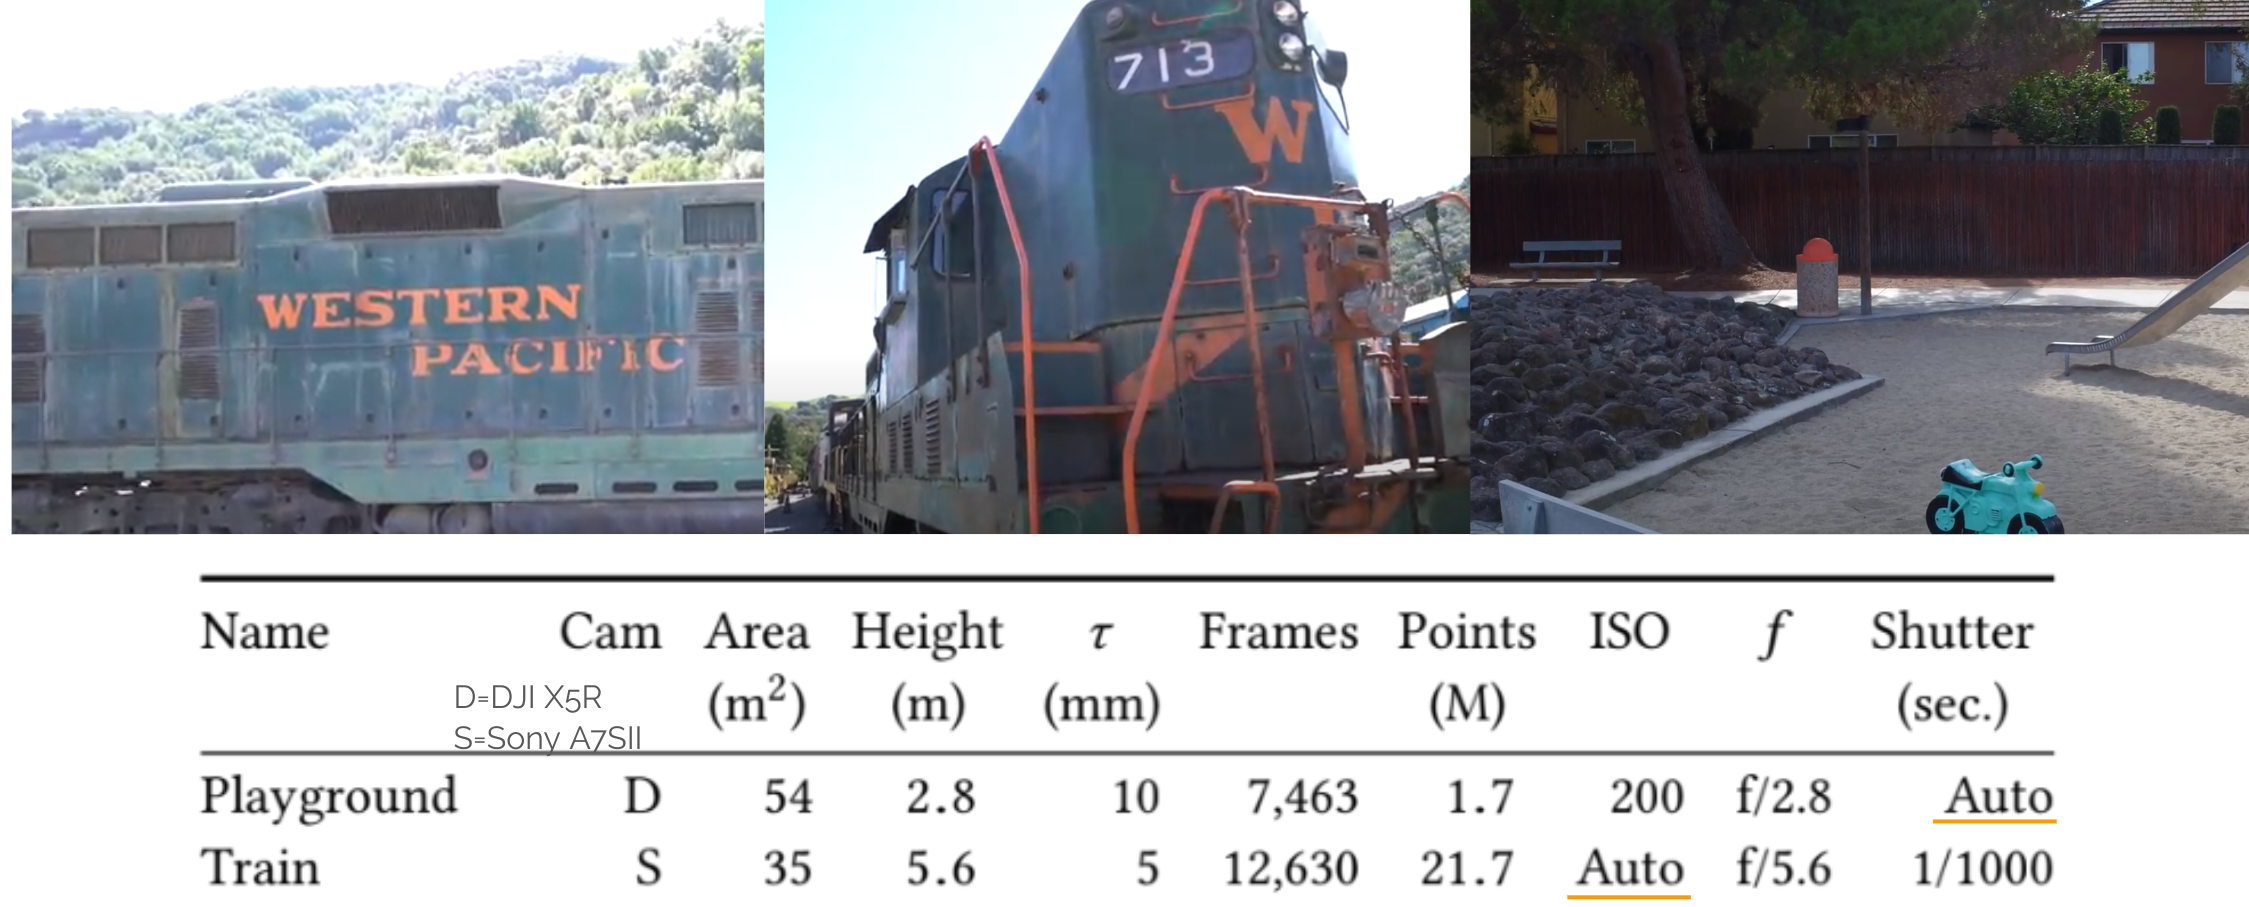
\includegraphics[width=6cm]{figures/tanks_and_temples.png}
    \caption{Information on the scenes captured for the Tanks and Temples dataset with high end video cameras in addition to a Lidar point cloud. On the left, the "train" scene shows clear signs of overexposure. The playground scene on the right has an overall correct and steady exposure}
    \label{fig:tank_and_temples}
\end{figure}


\noindent \textbf{switching to RAW format?} 
One of the potential way of creating a new benchmark would be to capture the scenes with a DSLR (like a full frame sensor) shot both in RAW and jpg (usually available on most cameras). RAW files would be post-processed by LightRoom or DxO Photolab with a neutral rendering: no tone mapping and neutral color rendering to get a Linear RGB set of images without any image compression. In case the sensor 12 or 14bits dynamic range is not sufficient, HDR captures could be achieved by bracketing. Intuitively, it sounds natural to use a tripod and merge the LDR linear images into a HDR linear image. But even handheld, all raw captures at various exposures could be used (let the alignment of bracketing images be implicitly done without any explicit need to merge exposures). These HDR images may serve as the ground truth for validation.

The main caveat of using RAW images is that there'll always be noise present proper to the camera sensor in the raw files. Since you get multiple views of the same scene, we can use the key concept proposed in Noise2Noise \cite{lehtinen2018noise2noise} that a neural network can be trained to denoise images without a ground truth images (it requires noisy burst of the same image instead). Here we have access to the same scene under different angles. The engine to implicity align them and get the right supervision is the rendering of the point cloud! This actual idea has been proposed in /cite{mildenhall2022rawnerf}
%TODO: Refer to NERF IN THE DARK

RGB (raw demosaicked) linear format is the only space in which an evaluation of the rendering quality does not depend on the camera ISP.
If one would really like to check the effect Training images could be either the jpgs or the reprocessed RAW files using a more scenic rendering: vibrancy to make some colors slightly more saturated (e.g. blue for skies but avoid saturating red too much for skin tones), tone mapping (global or local), sharpening / micro contrast.
